% ****** Start of file apssamp.tex ******
%
%   This file is part of the APS files in the REVTeX 4.2 distribution.
%   Version 4.2a of REVTeX, December 2014
%
%   Copyright (c) 2014 The American Physical Society.
%
%   See the REVTeX 4 README file for restrictions and more information.
%
% TeX'ing this file requires that you have AMS-LaTeX 2.0 installed
% as well as the rest of the prerequisites for REVTeX 4.2
%
% See the REVTeX 4 README file
% It also requires running BibTeX. The commands are as follows:
%
%  1)  latex apssamp.tex
%  2)  bibtex apssamp
%  3)  latex apssamp.tex
%  4)  latex apssamp.tex
%
\documentclass[%
reprint,
%superscriptaddress,
%groupedaddress,
%unsortedaddress,
%runinaddress,
%frontmatterverbose, 
%preprint,
%preprintnumbers,
%nofootinbib,
%nobibnotes,
%bibnotes,
 amsmath,amssymb,
 aps,
%pra,
%prb,
%rmp,
%prstab,
%prstper,
%floatfix,
]{revtex4-2}

\usepackage{graphicx}% Include figure files
\usepackage{dcolumn}% Align table columns on decimal point
\usepackage{bm}% bold math
\usepackage{float}
\usepackage{mathtools}
\usepackage{xcolor}
%\usepackage{hyperref}% add hypertext capabilities
%\usepackage[mathlines]{lineno}% Enable numbering of text and display math
%\linenumbers\relax % Commence numbering lines

%\usepackage[showframe,%Uncomment any one of the following lines to test 
%%scale=0.7, marginratio={1:1, 2:3}, ignoreall,% default settings
%%text={7in,10in},centering,
%%margin=1.5in,
%%total={6.5in,8.75in}, top=1.2in, left=0.9in, includefoot,
%%height=10in,a5paper,hmargin={3cm,0.8in},
%]{geometry}

\newcommand{\Hp}{\mathcal{H}}
\renewcommand{\thesection}{\arabic{section}}
\renewcommand{\thesubsection}{\arabic{subsection}}
\renewcommand{\thesubsubsection}{\arabic{subsubsection}}


\begin{document}

\section{Milestone I}

In this section we consider the evolution of the uniform background of the universe in the Lambda-Cold-Dark-Matter ($\Lambda$CDM) model which is considered to be the present day standard model of cosmology. The main goal of this section is to solve the unperturbed background evolution of the universe by using known cosmological parameters supplied by \cite{Planck:2018vyg} and comparing this to observational supernova data from \cite{SDSS:2014iwm}.

\subsection{Theory}
\subsubsection{Friedmann-Lema\^itre-Robertson-Walker}
In this milestone we approximate the universe to be completely isotropic and homogeneous over all scales. For large scales this has been shown to be a reasonable assumption from observations of the CMB power spectra \cite{dodelson:2003ft}. The universe must then satisfy a maximally symmetric metric. With some symmetry arguments, we arrive at an exact solution for the metric called the Friedmann-Lema\^itre-Robertson-Walker (FLRW) metric. In flat space, $k=0$, and Cartesian coordinates it is given by:
\[g_{\mu\nu}=\text{diag}\left[-1,a^2(t),a^2(t),a^2(t)\right],\]
where $a(t)$ is the scale factor, defined to be $1$ today, and we are using the mostly plus metric signature $(-,+,+,+)$. 

To make use of the line element above we consider the Einstein field equations (EFE):
\begin{equation}
	G_{\mu\nu}+\Lambda g_{\mu\nu}=8\pi G T_{\mu\nu},\label{eq:EFE}
\end{equation}
With the isotropy requirement, any stress-energy tensors which we will consider must be invariant under spatial rotations. To consider the general allowed form of the stress-energy tensor we decompose it as such:
\[T_{\mu\nu}(x)=\begin{bmatrix}
	T_{00}(x) & T_{0i}(x)\\
	T_{0i}(x) & \sigma_{ij}(x)
\end{bmatrix},\]
As usual, the $T_{00}=\rho$ component is to be interpreted as the energy density in a non-boosted frame. The requirement of homogeneity then imposes that one should not have any energy flux, as such finds $T_{0i}=0$. The isotropy requirement imposes that the matrix $\sigma$ must satisfy $R^T\sigma(x) R=\sigma(x)$ for all $x$ and rotation matrices $R$. The latter then implies that $[R,\sigma(x)]=0$. As the generators of the $SO(3)$ group form an algebra, Schurs' Lemma then states that this is satisfied iff $\sigma(x)\propto I\implies \sigma(x)=p(x)I$ for some function $p(x)$. Furthermore the homogeneity requirement imposes translation invariance, meaning that $p(x)=p(x+x_0)$. These requirements, a comoving observer, i.e. an observer in the rest frame of the universe, then implies that we may uniquely describe the universe as a perfect liquid with:
\[T_{\mu\nu}=(\rho+p)u_\mu u_\nu+g_{\mu\nu}p.\]
where $p$ is the pressure. As such, from the FRWL metric and the EFE one can derive the \textbf{Friedmann equations}:
\begin{align}
	\label{eq:F1}
	\left(\frac{\dot{a}}{a}\right)^2&\equiv H^2=\frac{8\pi G}{3}\rho,\\
	\label{eq:F2}
	\frac{\ddot{a}}{a}&=-\frac{4\pi G}{3}(\rho+3p),
\end{align}
where $\rho$ and $p$ are, as explained, the energy density and pressure respectively for a perfect liquid. 
\subsubsection{$\Lambda$CDM Model}
The $\Lambda$CDM model is derived by assuming; that we have some family of weakly interacting massive particles (WIMPs) which we call cold-dark-matter (CDM) and a cosmological constant, $\Lambda$, which accounts for the present day acceleration of the universe, which will be the dark energy in this article. The name CDM comes from assuming that they are massive enough to not be relativistic and hence cold. 
The first Friedmann equation (\ref{eq:F1}) can be rewritten such that the time dependence of the Hubble factor $H\equiv\dot{a}/a$ is given by:
\begin{equation}
	H^2=H_0^2\sum_i\Omega_{i0}a^{-3(1+\omega_i)},
	\label{eq:Hubblesquared}
\end{equation}
where $\omega_i\equiv p_i/\rho_i$ is the equation of state for the $i$-th particle type, $\Omega_i\equiv\rho_i/\rho_C$ is the relative energy density of the $i$-th particle type, $\rho_i$ is the energy density corresponding to the $i$-th particle type and $\sum_i\rho_i=\rho_C$ is the critical energy density required to have a flat universe which we observe today \cite{Planck:2018vyg}. We have that $\omega_{\text B}=0,\omega_{\text{R}}=1/3$ and $\omega_\Lambda=-1$ for baryons, relativistic particles (photons and massless neutrinos) and dark energy (DE) respectively. Simply plugging in the various particle types in (\ref{eq:Hubblesquared}) we have:
\begin{align}
	H=H_0\sqrt{\Omega_{\text M0}a^{-3}+\Omega_{\text{R}0}a^{-4}+\Omega_{\text K0}a^{-2}+\Omega_{\Lambda0}}, 
	\label{eq:Hubble}\\
	\Omega_{\text M0}\equiv \Omega_{B0}+\Omega_{\text{CDM}0},~~\Omega_{\text{R}0}\equiv \Omega_{\gamma0}+\Omega_{\nu0},\nonumber
\end{align}
where $\Omega_{B0},\,\Omega_{\text{CDM}0},\,\Omega_{\gamma0},\,\Omega_{\nu0}$ and $\Omega_{\Lambda0}$ are then the present day relative densities of baryonic matter (electrons \& protons), cold dark matter, radiation, neutrinos and dark energy respectively. The term $\Omega_{\text K0}=-kc^2/H_0$ denotes the curvature of the universe and encapsulates how said curvature affects expansion rates and energy densities. With the requirement for a flat universe we have that $\sum_i\Omega_i=1$ where $i$ refers to all non-curvature energy types. Since $\Omega_{\text B},\,\Omega_{\text{CDM}}$ and $\Omega_\gamma,\,\Omega_\nu$ give the same contribution to the time evolution of the Hubble parameter, we will often bundle these together as ``matter'' and ``radiation'' (or ``relativistic'') particles respectively as was done in (\ref{eq:Hubble}).

The other Friedmann equation (\ref{eq:F2}), together with each particles equation of state, is then used to describe how each component evolves with time:
\begin{alignat}{2}
	\Omega_{\text B}(a)&=\frac{\Omega_{\text B0}}{a\Hp^2/H_0^2},\hspace{3.5mm}\Omega_{\text{CDM}}(a)&&=\frac{\Omega_{\text{CDM}0}}{a\Hp^2/H_0^2},\nonumber\\
	\Omega_{\gamma}(a)&=\frac{\Omega_{\gamma0}}{a^2\Hp^2/H_0^2},\hspace{7mm}\Omega_{\nu}(a)&&=\frac{\Omega_{\nu0}}{a^2\Hp^2/H_0^2},\label{eq:Omegai}\\
	\Omega_{\text K}(a)&=\frac{\Omega_{\text K0}}{\Hp^2/H_0^2},\hspace{10mm}\Omega_{\Lambda}(a)&&=\frac{\Omega_{\Lambda0}}{H^2/H_0^2},\nonumber
\end{alignat}
where $\Hp\equiv aH$ is the \textbf{conformal Hubble factor}. 
Two of the six density parameters follow from the observed temperature of the CMB and are given by:
\begin{align}
	\label{eq:ORad}
	\Omega_{\gamma0}&=\frac{8\pi^3 G}{45 H_0^2}\frac{(k_BT_{\text{CMB}0})^4}{\hbar^3 c^5},\\
	\label{eq:ONu}
	\Omega_{\nu0}&=\Omega_{\gamma0}N_{\text{eff}}\cdot\frac{7}{8}\left(\frac{4}{11}\right)^{4/3},
\end{align}
where $T_{\text{CMB}0}$ is the temperature of CMB photons today and $N_{\text{eff}}=3.046$ is the effective number of massless neutrinos. \cite{Planck:2018vyg}

The $\Lambda$CDM model is then fully determined by these cosmological observables which come from 2018 Planck \cite{Planck:2018vyg}:
\begin{alignat}{2}
	\frac{H_0\,\text{Mpc}}{100\,\text{km/s}}\equiv h &= 0.67,\hspace{12.2mm}N_\text{eff}&&=3.046,\nonumber\\
	\Omega_{\text B0}&=0.05,\hspace{7.3mm}\Omega_{\text{CDM}0}&&=0.267,\label{eq:planck_data}\\
	\Omega_{\text K0}&=0.00,\hspace{8mm}T_{\text{CMB}0}&&=2.7255.\nonumber
\end{alignat}
\subsubsection{Time and Distance Measurements in Cosmology}
Since the expansion of the universe is strictly positive w.r.t. time, the scale factor $a(t)$ is an injective function and can thus be used as a time measurement. In this paper we will, for computational purposes, be using the variable $x\equiv\ln(a)\implies a=e^x$. 

Again, due to the expansion of the universe, one can also measure how much the wavelength of a photon released at initial time $t_i$ has stretched before it reaches us at final time $t_f$, commonly known as the \textbf{redshift}:
\[z=e^{x(t_f)-x(t_i)}-1.\]
A derivation can be found in \cite{Davis_2004}. Since we are mainly interested in the redshift w.r.t. today then $x(t_f)=0$. Thus the formula which will be used in this article is $z=e^{-x(t_i)}-1$.

Further we consider the \textbf{horizon}, i.e. the ``distance'' massless particles may have travelled since the big bang. Since the universe is expanding, this will be appreciably larger than $ct$. Considering a time $t_1$, light would have travelled a distance $d_1>ct_1$. We can then consider what $t_1$ must be such that this becomes an equality. For this we define the \textbf{conformal time} $d\eta=dt/a$ (or conformal distance with the appropriate insertion of $c$) which can be rewritten as $\eta(t)\equiv\int_0^t\frac{c}{a}dt'$ and we get the differential equation:
\begin{equation}
	\frac{d\eta}{dx}=\frac{c}{\Hp},\label{eq:detaODE}
\end{equation}
along with the initial condition $\eta(-\infty)=0$, which can be solved analytically in the radiation dominated era. We will then use the analytical solution to approximate that at some very early time, $x_\text{start}$ such that we have the new initial condition $\eta(x_\text{start})=c/\Hp(x_\text{start})$ where we will solve onwards numerically. 

A useful distance measure is the \textbf{comoving distance} $\chi$ which is derived by the FLRW metric:
\[\chi=\int_{t_i}^{t_0}dt\frac{c}{a}=\int_1^ada'\frac{c}{a'^2H}=\int_0^zdz'\frac{c}{H}=\eta-\eta_0.\]
Considering a light-like path with the FLRW metric in curved space one arrives at the \textbf{proper distance} $r$:
\[
r=
\begin{cases}
	\,\chi\frac{\sin(\sqrt{\left|\Omega_{\text K0}\right|}H_0\chi/c)}{\sqrt{\left|\Omega_{\text K0}\right|}H_0\chi/c},& \Omega_{\text K0}<0~\text{``Closed''}\\
	\,\chi, & \Omega_{\text K0}=0~\text{``Flat''}\\
	\,\chi\frac{\sinh(\sqrt{\left|\Omega_{\text K0}\right|}H_0\chi/c)}{\sqrt{\left|\Omega_{\text K0}\right|}H_0\chi/c},& \Omega_{\text K0}>0~\text{``Open''}
\end{cases}.
\]
We then consider the angular \textbf{diameter distance} $d_A=\Delta s/\Delta \theta$ where $\Delta s$ is the objects physical size and $\Delta \theta$ its angular size as viewed from Earth. Once again from the FRLW metric, now in spherical coordinates:
\[ds^2=-c^2dt^2+a^2(dr^2+r^2d\theta^2+\sin^2\theta d\phi^2),\]
one can find that this can be expressed in terms of our cosmological parameters as $d_A=ar$. The \textbf{luminosity distance} $d_L$ is defined from $d_L=\sqrt{\frac{L}{4\pi F}}$ where $L$ is the intrinsic luminosity and $F$ is the measured flux. As implied by its name, this quantity is related to $d_A$ by $d_L=d_A/a^2=r/a$. 

At last we consider the \textbf{cosmic time} $t$ in our $x$ coordinate:
\[t(x)=\int_0^a\frac{da}{aH}=\int_{-\infty}^0\frac{dx}{H(x)}.\]
From this we get to the ODE:
\begin{equation}
	\frac{dt}{dx}=\frac{1}{H}, \label{eq:dtdx}
\end{equation}
with the initial condition $t(-\infty)=0$. This initial condition states that cosmic time begins once the big bang happened. As before, we make an analytical approximation which gives us the initial condition $t(x_\text{start})=\frac{1}{2H(x_\text{start})}$ and solved numerically from here.

\subsubsection{Markov-Chain Monte Carlo Method}
In this milestone one of the major computational method which will be used is the Markov Chain Monte Carlo (MCMC) method. The particular algorithm we use is the Metropolis algorithm which generates a Markov chain, where in each step, the chain corresponds to a proposed set of model parameters, which in our case are $h, \Omega_{\text M0}$ and $\Omega_{\text K0}$. These parameters are sampled from a probability distribution guided by certain priors, i.e. accepted ranges, where data outside of these priors are omitted. The algorithm then eventually converges to the posterior distribution of the parameters given the observed data. This can then be used to constrain the cosmological parameters, in which we decide to focus on $h, \Omega_{\text{CDM}0}$ and $\Omega_{\text M0}$. A $\chi^2$-test is then done by the assumption that the measurements are Gaussian distributed and uncorrelated between different redshift. The likelihood function is then given by $L\propto e^{-\chi^2/2}$ where:
\[\chi^2(h,\Omega_{\text M0},\Omega_{\text K0})=\sum_{i=1}^N[d_L(z_i,h,\Omega_{\text M0},\Omega_{\text K0})-d_L^\text{obs}]^2/\sigma_i^2.\]
Here $\sigma_i$ is the standard deviation for the $i$-th data point and $N$ is the total number of data points. The set of parameters with the highest likelihood is our best-fit model, which also happen to be the values which minimize $\chi^2$. To check that this best-fit is in fact a good fit one can consider a set of data points which all lie exactly $1\sigma$ away from the observed values. As such the expression in the sum simply reduces to $1$. Thus when summing over $N$ terms equal to $1$ we would have that $\chi^2/N=1$. Hence we will consider a best-fit to be a good fit if $\chi^2\sim N$. For the case when $\chi^2\ll N$ then we over-fit the model, meaning we may be capturing random noise and fluctuations in the data, whilst if $\chi^2\gg N$ then we simply have a bad correspondence with the data and/or underlying assumptions (such as the assumption that the measurements are Gaussian).

\subsection{Implementation details}
\subsubsection{Solving the ODEs}
To implement some numerical tools to solve for the background we first implement the data from (\ref{eq:planck_data}) and computed the derived quantities $\Omega_{\gamma0}$ and $\Omega_{\nu0}$ with (\ref{eq:ORad},\ref{eq:ONu}), and $\Omega_{\Lambda0}=1-\Omega_\text{rest0}$ where ``rest'' refers to all the other $\Omega_i$.  

Next we implemented an ordinary differential equation (ODE) solver to solve the ODEs for $\eta(x)$ and $t(x)$. This was done by first setting up the respective differential equation (\ref{eq:detaODE},\ref{eq:dtdx}) with its corresponding initial condition, then an ODE solver was used to get a result which was then splined. The ODE solver and splining programs were already provided in the template. 

Further we computed $H(x)$ from (\ref{eq:Hubble}) which was used together with the various relations from the theory section to compute $\Hp,\frac{d\Hp}{dx},\frac{d^2\Hp}{dx^2},\Omega_i,r,d_A,d_L,\chi$ and $T_{\text{CMB}}$ all as a function of our time variable $x$. Note that the expressions for $\frac{d\Hp}{dx}$ and $\frac{d^2\Hp}{dx^2}$ were found analytically from \ref{eq:Hubble}. The calculated data was then written to data files to be analyzed in Python.
\subsubsection{MCMC fit}
We then compared our numerical data  for the luminosity distance $d_L$ to observational data from \cite{SDSS:2014iwm}, containing $N=31$ data points, by performing an MCMC fit. The upper and lower priors which were used are $\{1.5,1,1\}$ and $\{0.5,0,-1\}$ for $h, \Omega_{\text M}$ and $\Omega_{\text K}$ respectively. The algorithm then computes an initial $\chi^2$ with some randomly generated parameters. It repeats this process and checks whether the new $\chi^2_\text{new}$ is less than the old $\chi^2_\text{old}$. If this is the case then it accepts this sample and starts again. However if this previous test is not the case we then perform a random check $e^{-(\chi^2_\text{new}-\chi_\text{old}^2)/2}>u$ where $u$ is number drawn from a uniform distribution in the interval $[0,1]$. If it passes this test then $\chi^2_\text{new}$ is accepted and the process carries on. This additional test is the main part of the Metropolis algorithm and is done to capture the full posterior probability distribution function (PDF) of the various parameters.  As before, the data was printed to a data file and imported to Python.
\subsubsection{Python}
$x$-values corresponding to radiation-matter- and matter-DE-equality were found by finding running a script over the data to find where the absolute value of the difference $|\Omega_i-\Omega_j|=0$. In reality they were never quite 0 due to running over a discrete index, thus we simply set some low threshold, e.g. $5\cdot10^{-5}$. To find when the universe accelerates we note that:
\[\Hp=\frac{\dot a}{a}a=\dot a\implies \frac{d\Hp}{dx}=\frac{d\Hp}{dt}\frac{dt}{dx}=\ddot{a}\frac{dt}{dx},\]
and from (\ref{eq:dtdx}) we then have:
\[\frac{d\Hp}{dx}\equiv\Hp'=\frac{\ddot a}{H}.\]
Since $H$ is strictly positive we can then look at when $\Hp'$ changes from negative to positive. So again a Python script which runs over the indices of $\Hp$ were used to find which $x$-values this sign change happened, which corresponds to where the universe began to accelerate. 

The MCMC-fit was then analyzed and a scatterplot in the $\Omega_\Lambda\Omega_\text M$-plane was created with the $(1\sigma,2\sigma)$ confidence regions $\chi^2-\chi^2_\text{min}<(3.53,8.02)$ respectively. These particular values were found from common $\chi^2$ distribution tables with $k=3$ degrees of freedom. A histogram of the PDF  from the accepted samples of $h$ along with a Gaussian fit was along with a comparison of our theoretical $d_L$ vs. the real supernova data were also plotted.

\subsection{Tests of data}

Before considering the results it is reasonable to conduct some sanity checks on the data to make sure everything was implemented correctly. To check that the data is consistent with the analytical expressions we consider the following quantities analytically in the different regimes:
\[\frac{\Hp'}{\Hp},\hspace{5mm}\frac{1}{\Hp}\frac{d^2\Hp}{dx^2}\equiv\frac{\Hp''}{\Hp},\hspace{5mm}\frac{1}{c}\eta\Hp.\]
\subsubsection{$\Hp'$ and $\Hp''$}
In the radiation dominated era where we approximate $\Omega_{\text{R}}\approx1\implies\Omega_\text{rest}\approx0$. Then by using (\ref{eq:Hubble}) we find:
\begin{alignat*}{2}
	H_{\text{R}}(x)&\approx H_0,~~\Hp_{\text{R}}(x)&&\approx H_0e^{-x},\\
	\frac{\Hp_{\text{R}}'}{\Hp_{\text{R}}}&\approx-1,\hspace{6.5mm}\frac{\Hp_{\text{R}}''}{\Hp_{\text{R}}}&&\approx1,
\end{alignat*}
and similarly using the approximations $\Omega_{\text M}\approx1$ and $\Omega_\Lambda\approx1$ respectively, we get:
\begin{alignat*}{2}
	H_\text{M}(x)&\approx H_0e^{x/2},\hspace{5mm}\Hp_\text M(x)&&\approx H_0e^{-x/2},\\
	\frac{\Hp_\text M'}{\Hp_\text M}&\approx-1/2,\hspace{12mm}\frac{\Hp_\text M''}{\Hp_\text M}&&\approx1/4,\\
	H_\Lambda(x)&\approx H_0,\hspace{12.5mm}\Hp_\Lambda(x)&&\approx H_0e^{x},
\end{alignat*}
\vspace{-7.2mm}
\[\frac{\Hp_\Lambda'}{\Hp_\Lambda}\approx\frac{\Hp_\Lambda''}{\Hp_\Lambda}\approx1.\]
Plotting these assumptions with the data we have FIG. \ref{fig:dHpddHp_vs_anal}. We see that there is a reasonable agreement with the analytical approximations in the given regimes. As we will see in later, $\Omega_{\text M}\approx1$ is a relatively poor approximation compared to the others, hence larger a deviation is to be expected.
\begin{figure}[ht!]
	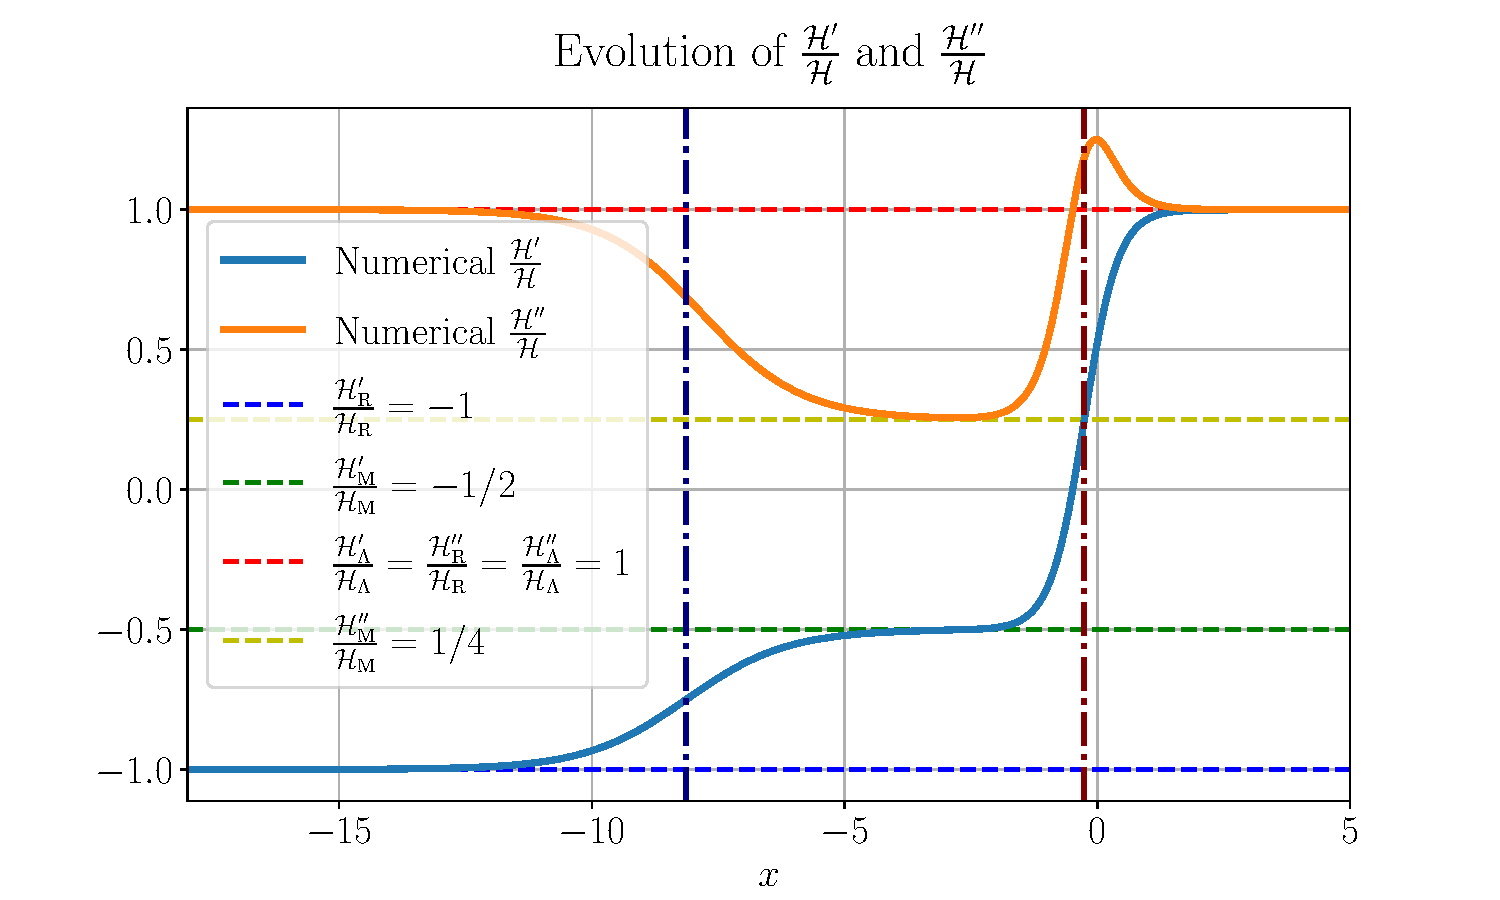
\includegraphics[width = \linewidth]{Figures/dHpddHp_vs_anal.pdf}
	\caption{$\Hp'/\Hp$ and $\Hp''/\Hp$ compared to analytical approximations in the various regimes where the left and right dash-dotted vertical lines signify radiation-matter equality and matter-dark energy equality respectively.}
	\label{fig:dHpddHp_vs_anal}
\end{figure}
\subsubsection{Conformal Time}
Analytical approximations for the conformal time requires a little more effort. For the radiation dominated era we can solve (\ref{eq:detaODE}) analytically:
\[\eta_\text{R}(x)=\int_{-\infty}^x\frac{c}{\Hp_\text{R}}dx'\approx\int_{-\infty}^x\frac{c}{H_0}e^{x'}dx'=\frac{c}{H_0}e^x.\]
Now we approximate this radiation dominated epoch to end abruptly at some time $x_1$ such that we can write the conformal time in the matter dominated epoch as:
\begin{align*}
	\eta_\text M(x)&\approx\eta_\text{R}(x_1)+\int_{x_1}^x\frac{c}{\Hp_\text M}dx'\\
	&\approx\frac{c}{H_0}\left(e^{x_1}+\int_{x_1}^xe^{x'/2}dx' \right)\\
	&=\frac{c}{H_0}(e^{x_1}-2e^{x_1/2}+2e^{x/2}).
\end{align*}
Again we assume that the matter dominated epoch ends abruptly at some time $x_2$ such that we can approximate:
\begin{align*}
	\eta_\Lambda(x)&\approx\eta_\text M(x_2)+\int_{x_2}^\infty\frac{c}{\Hp_\Lambda}dx'\\
	&\approx\frac{c}{H_0}\left(e^{x_1}-2e^{x_1/2}+2e^{x_1/2}+\int_{x_2}^x e^{-x'}dx' \right)\\
	&=\frac{c}{H_0}\left(e^{x_1}-2e^{x_1/2}+2e^{x_2/2}+e^{-x_2}-e^{-x} \right).
\end{align*}
Thus we find that for the various regimes we have:
\begin{align*}
	\eta_\text{R}\Hp_\text{R}/c&\approx1,\\
	\eta_\text M\Hp_\text M/c&\approx(e^{x_1}-2e^{x_2/2}+2e^{x/2})e^{-x/2},\\
	\eta_\Lambda\Hp_\Lambda/c&\approx(e^{x_1}-2e^{x_1/2}+2e^{x_2/2}+e^{-x_2}-e^{-x})e^{x}.
\end{align*}
Using the $x$ values corresponding to $\Omega_{\text{R}}=\Omega_\text M$ and $\Omega_{\text M}=\Omega_\Lambda$ as the time where the respective epochs start and end we get the upper graph in FIG. \ref{fig:eta_vs_anal_merge}.
\begin{figure}[ht!]
	\caption{Numerical $\eta\Hp/c$ compared to analytical approximations in the various regimes where epochs are approximated to abruptly once $\Omega_i=\Omega_j$.}
	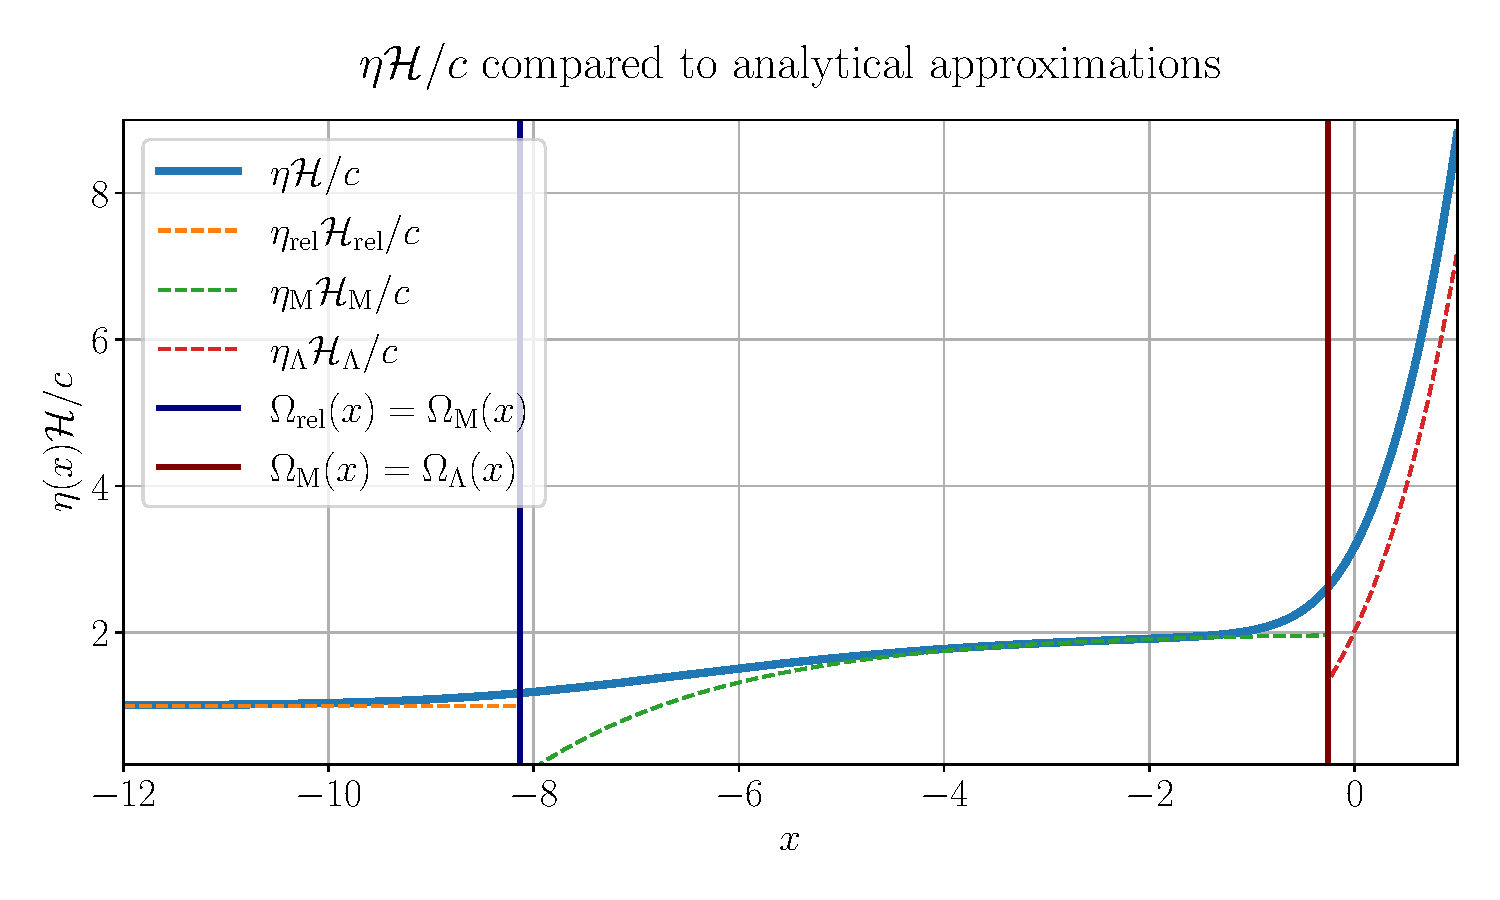
\includegraphics[width = \linewidth]{Figures/Eta_vs_anal_merge.pdf}
	\label{fig:eta_vs_anal_merge}
\end{figure}
Clearly this approximation will be nothing close to exact due to the assumption that the epochs end abruptly when in reality the epoch's change continuously and relatively slowly. Since $\eta$ depends on how long the previous epochs lasted we can see that this heavily affects the final epoch. 

Overall the data seems to be consistent with the analytical expressions, even if the conformal time is a rather difficult parameter to define a robust approximation for.

\subsection{Results}

Now that the data has been stress tested to show that they are at least valid in certain regions we can go on to look at some of the results.
\subsubsection{Time Evolution of  Cosmic Parameters}
We first consider the time evolution of the various relative energy densities $\Omega_i$ as a function of the scale factor $a(t)$ as given in FIG. \ref{fig:Omegai}.
\begin{figure}[ht!]
	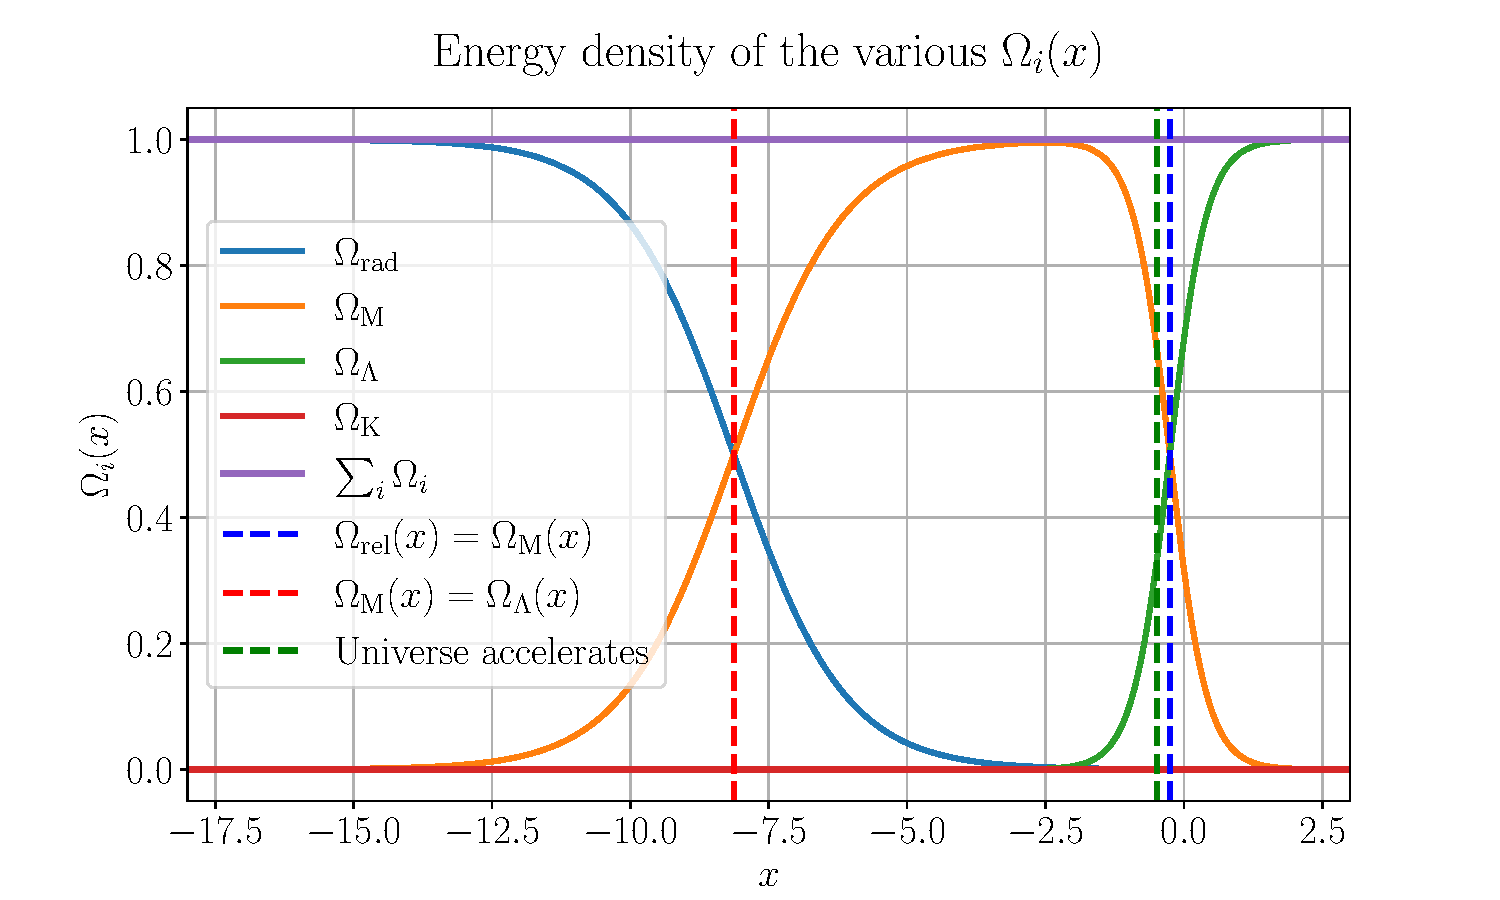
\includegraphics[width = \linewidth]{Figures/Omega_i.pdf}
	\caption{Time evolution of the density parameters $\Omega_i$ as a function of the scale factor $a$.}
	\label{fig:Omegai}
\end{figure}

Here we can clearly see the different regimes of the various quantities. The early universe is in a complete radiation domination at early times which implies that the universe expands $a(t)\propto t^{1/2}$. The universe then relatively slowly switches over to becoming matter dominated as time passes. For a short period of time we have complete matter domination, implying an expansion $a(t)\propto t^{2/3}$. Then dark energy starts to dominate at later times, causing the universe to begin to accelerate, until we get the known result of today where dark energy accounts for roughly 68\% of the total energy in the universe today. It then further predicts that in the future, dark energy domination will continue to grow as time passes.

The time evolution of the conformal Hubble factor $\Hp(x),$ cosmic time $t(x)$ and conformal distance $\eta(x)/c$ is given in FIG. \ref{fig:TimeEvHp}. The notable acceleration at later times in the $\Hp$ plot can be seen by when the derivative of $\Hp$ changes sign as mentioned previously. One can also see that this same phenomena affects both the cosmic time and conformal distance inversely at the same time. This is due to them both being inversely proportional to the conformal Hubble factor.
\begin{figure}[ht!]
	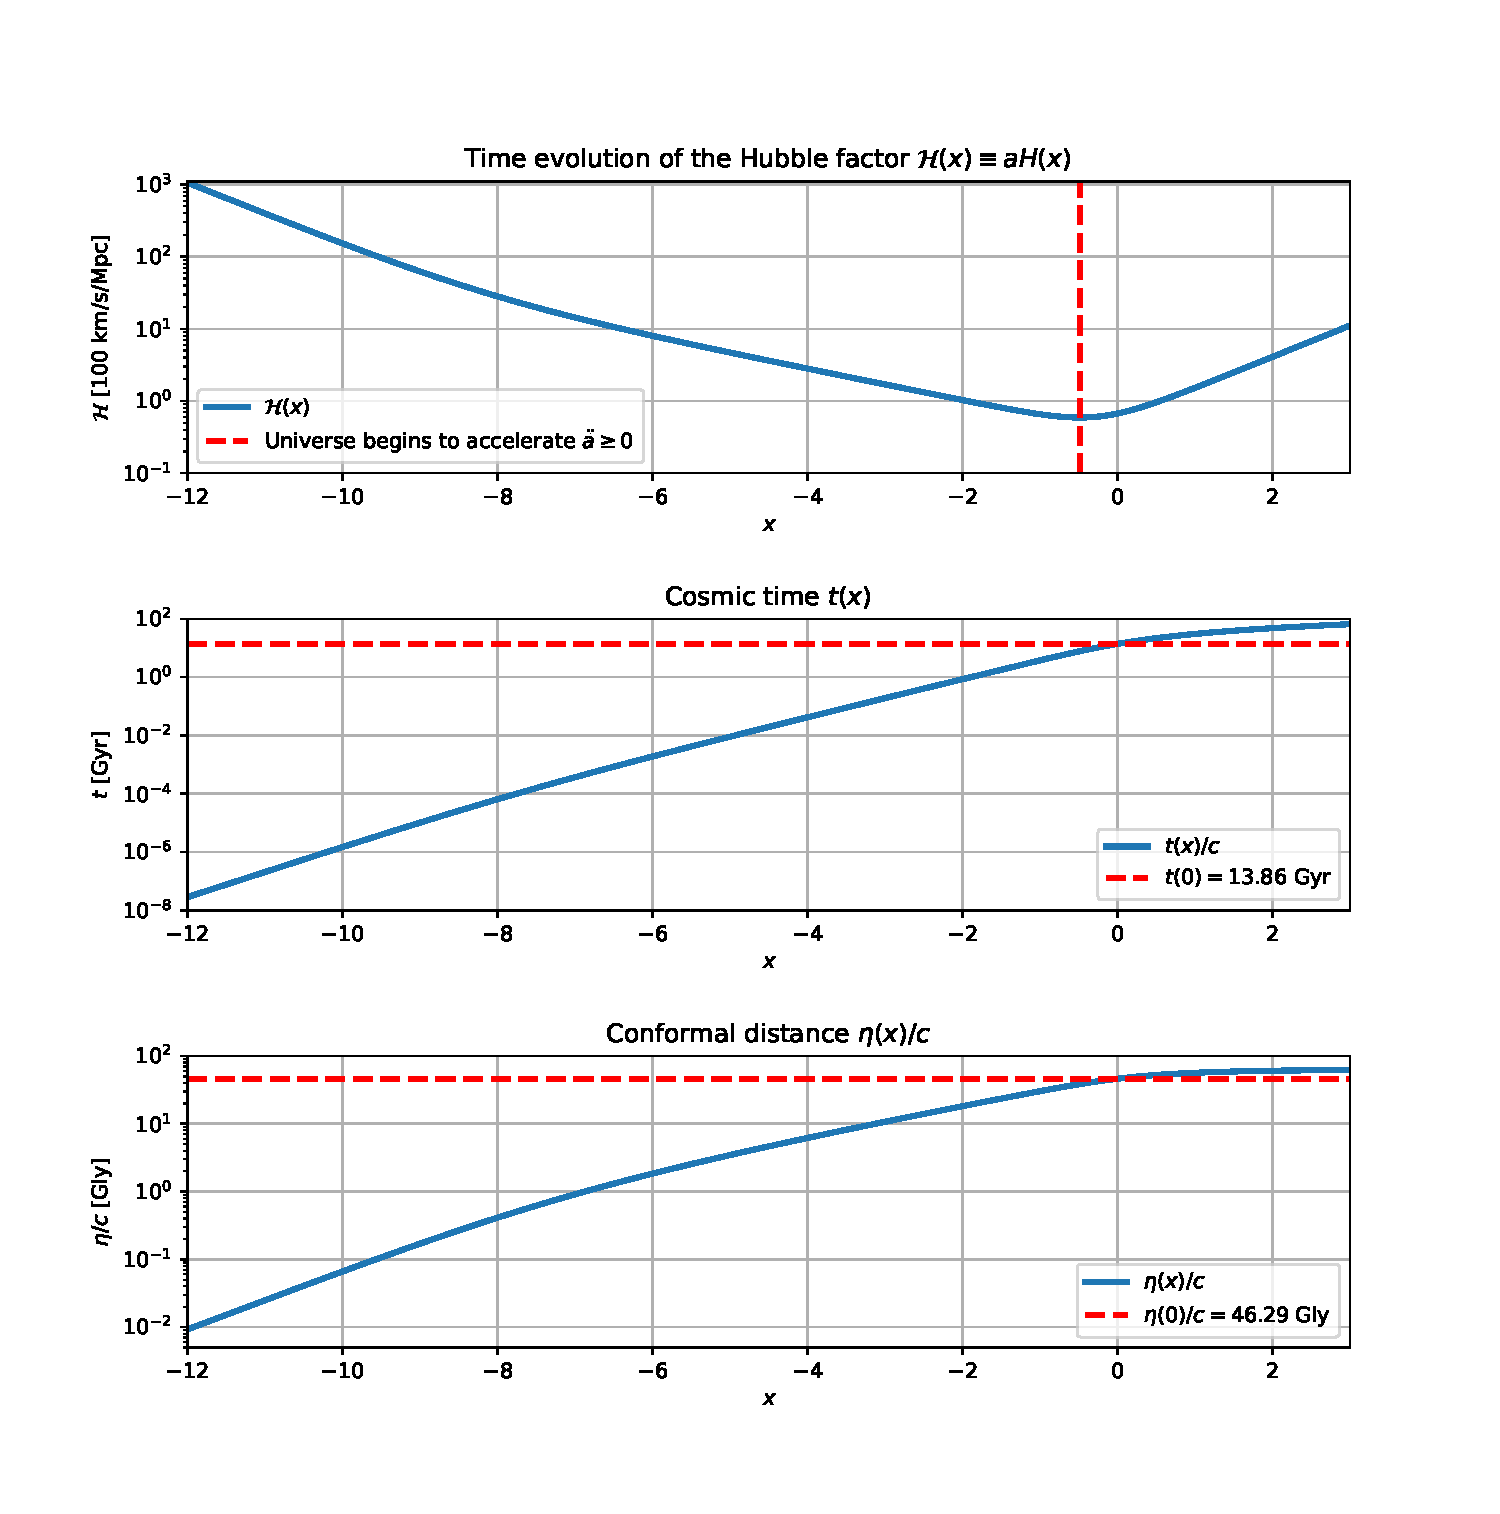
\includegraphics[width = \linewidth]{Figures/merge_Hp_t_eta_Ev.pdf}
	\caption{Time evolution of the conformal Hubble factor $\Hp$, cosmic time $t$ and conformal distance $\eta/c$ as a function of $x$.}
	\label{fig:TimeEvHp}
\end{figure}

Next we consider the values of $x,z,t,\eta,\Omega_\text M, \Omega_\Lambda$ and $\Omega_\text R$ at various important events. A summary of these events is given in TABLE \ref{tab:cosmo_events}.
\renewcommand{\arraystretch}{1.25}
\begin{table*}[ht!] % Neither this, nor transpose of the table with reduced headers fit single-column :'(
	\caption{Results for cosmological parameters at various important events from numerical data.}
	\begin{tabular}{|l|c|c|c|c|c|c|c|}
		\hline
		Event & $x$ & $z(x)$ & $t(x)$ [Gly] & $\eta(x)/c$ [Gly] & $\Omega_\text M$ & $\Omega_{\Lambda}$ & $\Omega_{\text{Rel}}$ \\
		\hline
		Radiation-Matter Equality  & $-8.132$ & $3401$ & $5.106 \cdot 10^{-5}$ & $0.368$ & $0.500$ & $2.737 \cdot 10^{-11}$ & $0.500$ \\
		\hline
		Universe Accelerates & $-0.486$ & $0.626$ & $7.761$ & $38.55$ & $0.666$ & $0.334$ & $3.183\cdot10^{-4}$ \\
		\hline
		Matter-DE Equality & $-0.256$ & $0.292$ & $10.38$ & $42.33$ & $0.500$ & $0.500$ & $1.900\cdot10^{-4}$ \\
		\hline
		Universe Today & $\phantom{-}0.000 $ & $0.000 $ & $13.86$ & $46.29$ & $0.317$ & $0.683$ & $9.320 \cdot 10^{-5}$ \\
		\hline
	\end{tabular}
	\label{tab:cosmo_events}
\end{table*}

Here we can see that radiation-matter-equality happened roughly $51000$ years after the big bang. Further, the universe begins to accelerate roughly 7.7 billion years after the big bang. One may notice that this happens $2\Omega_{\Lambda}\approx\Omega_{\text M}$ and $\Omega_{\text{others}}\approx0$. We can check this analytically by considering these approximation. We have that $\Omega_{\text{tot}}\approx3\Omega_{\Lambda}$ and hence $\rho_\text{tot}=3\rho_\Lambda$. Further we have that $p_\text{tot}=p_\Lambda+p_\text{M}=p_\Lambda$ due to $p_\text{M}=0$ from its equation of state. Inserting this into the Friedman equation (\ref{eq:F2}) with the relevant equation of state we get:
\begin{align*}
	\frac{\ddot{a}}{a}&\approx -\frac{4\pi G}{3}(3\rho_\Lambda+3(p_\Lambda+p_\text{M}))\\
	&=-\frac{4\pi G}{3}(3\rho_\Lambda-3\rho_\Lambda)=0
\end{align*}
Now, since $a$ is strictly a positive number then, mathematically, all that remains to check whether this is not when deceleration starts or a terrace point. To ensure this one can just check some arbitrarily close points such as $\Omega_{\Lambda}=1/3\pm\epsilon$ and $\Omega_{\text M}=2/3\mp\epsilon$ where $\epsilon$ is some tiny positive number.

Next in the table we have $t(x=0)$ which corresponds to the age of the universe today. \cite{Planck:2018vyg} estimates this to be $13.78\pm0.20\,$Gly which is reasonably close to our value of $13.86\,$Gly. Similarly $\eta(x=0)$ shows us the actual size of the observable universe today. \cite{Gott:2003pf} states the expected conformal distance of the universe is roughly $14\,$Gpc which corresponds to $45.7\,$Gly, again in reasonable agreement with the data. 
\subsubsection{Supernova Comparison}
Further we compare our numerical data to data collected from supernova observations \cite{SDSS:2014iwm} by; comparing the luminosity distance is given in FIG. \ref{fig:LumiDistance} and making a posterior probability distribution function (PDF) of the Hubble parameter $H_0$ in FIG. \ref{fig:PDEh}. We note that the found $\chi^2_\text{min}=29.3$ for the MCMC fit, which then yields that for the points accepted within the $1\sigma$ region follow $\chi^2\sim N$ to a very good approximation, suggesting that we have a good fit. 

The luminosity distance from the observational data is seemingly always lower than our data. This phenomena is known as the \textbf{Hubble tension} which is a widely known problem in today's standard model of cosmology \cite{Di_Valentino_2021}. Direct data, such as supernova data, seemingly always prefers lower values for luminosity distance, and thus, higher values for $h$ that can be seen in FIG. \ref{fig:PDEh}. Indirect data, such as the CMB, however prefer higher values for $d_L$ and thus lower values $h$ with much smaller error-bars. This is an ongoing issue which suggests that the $\Lambda$CDM model is not a complete model and must be modified. The posterior PDF of the Hubble parameter today $H_0$ shows that the Gaussian fit is centered at roughly $70.1\,\text{km/s/Mpc}$. As mentioned, this is a large discrepancy from $H_0=67\,\text{km/s/Mpc}$ which we got from the fiducial cosmology but still considered a common result from direct data. 


\begin{figure}[ht!]
	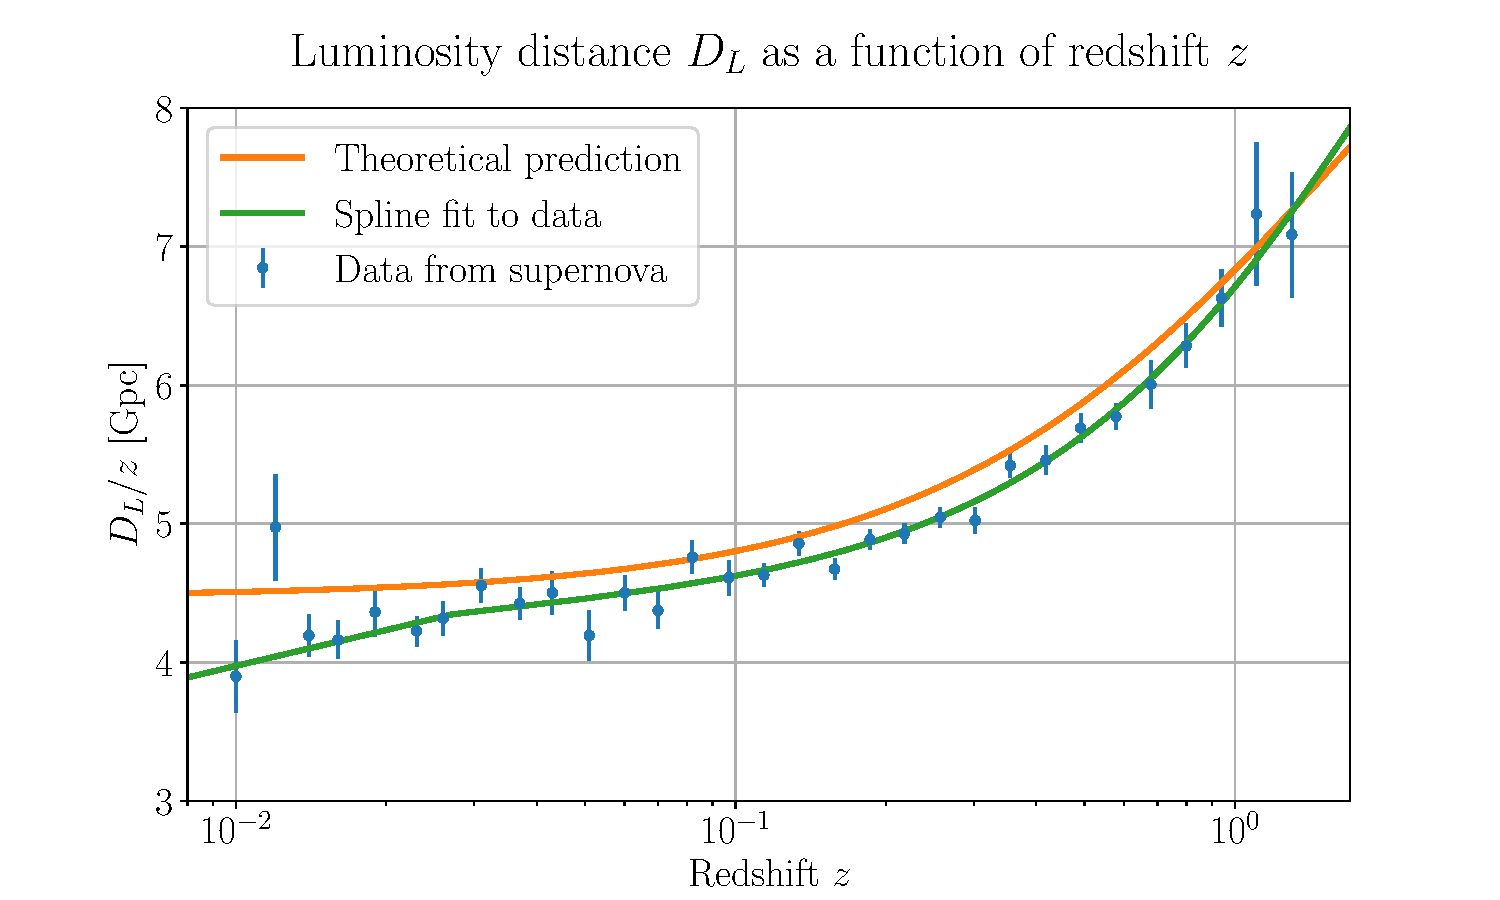
\includegraphics[width = \linewidth]{Figures/LumiDistance.pdf}
	\caption{Luminosity distance over redshift $z$, plotted against redshift $z$ for both; our numerical data, and observational data from Betoule et. al. \cite{SDSS:2014iwm} with error-bars.}
	\label{fig:LumiDistance}
\end{figure}
\begin{figure}[ht!]
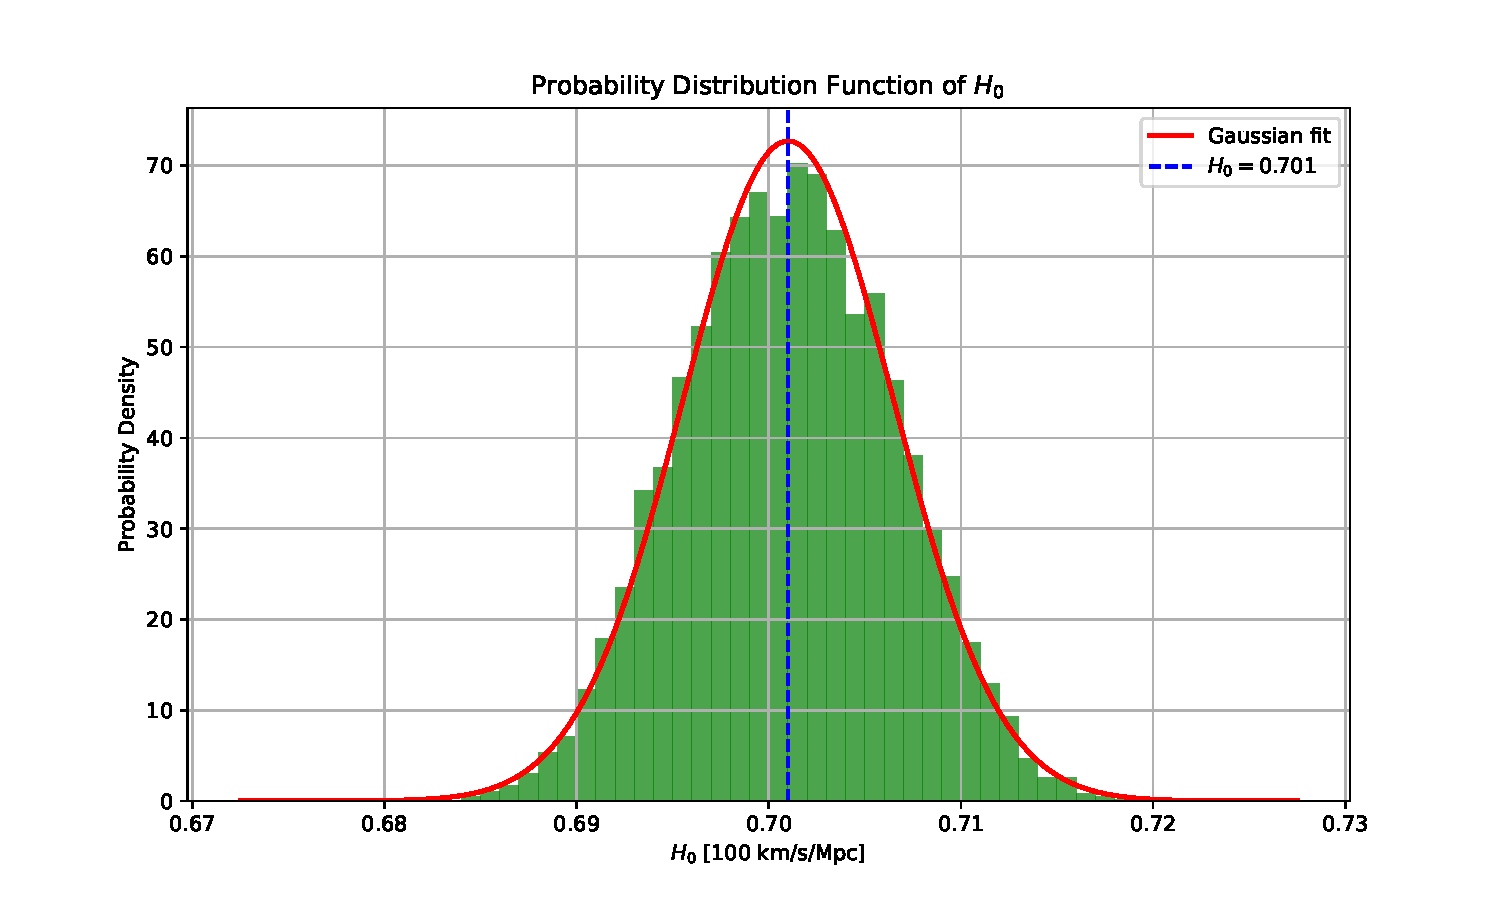
\includegraphics[width = \linewidth]{Figures/PDEh.pdf}
\caption{Posterior PDF of the Hubble parameter $H_0$ compared to the fiducial value $H_0=67\,$km/s/Mpc.}
\label{fig:PDEh}
\end{figure}

Next we consider the scatterplot in the $\Omega_\Lambda\Omega_\text M$-plane shown in FIG. \ref{fig:scatt}. The scatter-plot helps us visualize the degeneracy between the density parameters, i.e. that many different combinations of $\Omega_\text M$ and $\Omega_{\Lambda}$ can yield similar observational results. This leads to rather large degenerate regions in the parameter space. In this figure we can see that the flat universe constraint significantly reduces this degeneracy by lowering the allowed parameters by multiple orders of magnitude. The figure clearly shows that $\Omega_{\Lambda0}=0$ is completely excluded given the observational data as this would be far outside the $2\sigma$ constraint. The best-fit value for $\Omega_{\text K0}=0.067$ tells us that the universe is seemingly quite flat, but that there is indeed some curvature. To test out whether this might just be an insensitivity to the $\Omega_{\text K0}$ parameter the code was run again with a large initial value $\Omega_{\text K0}$. The result did not seem to change whatsoever and thus this implies that our model is insensitive to the curvature of the universe.

\begin{figure}[ht!]
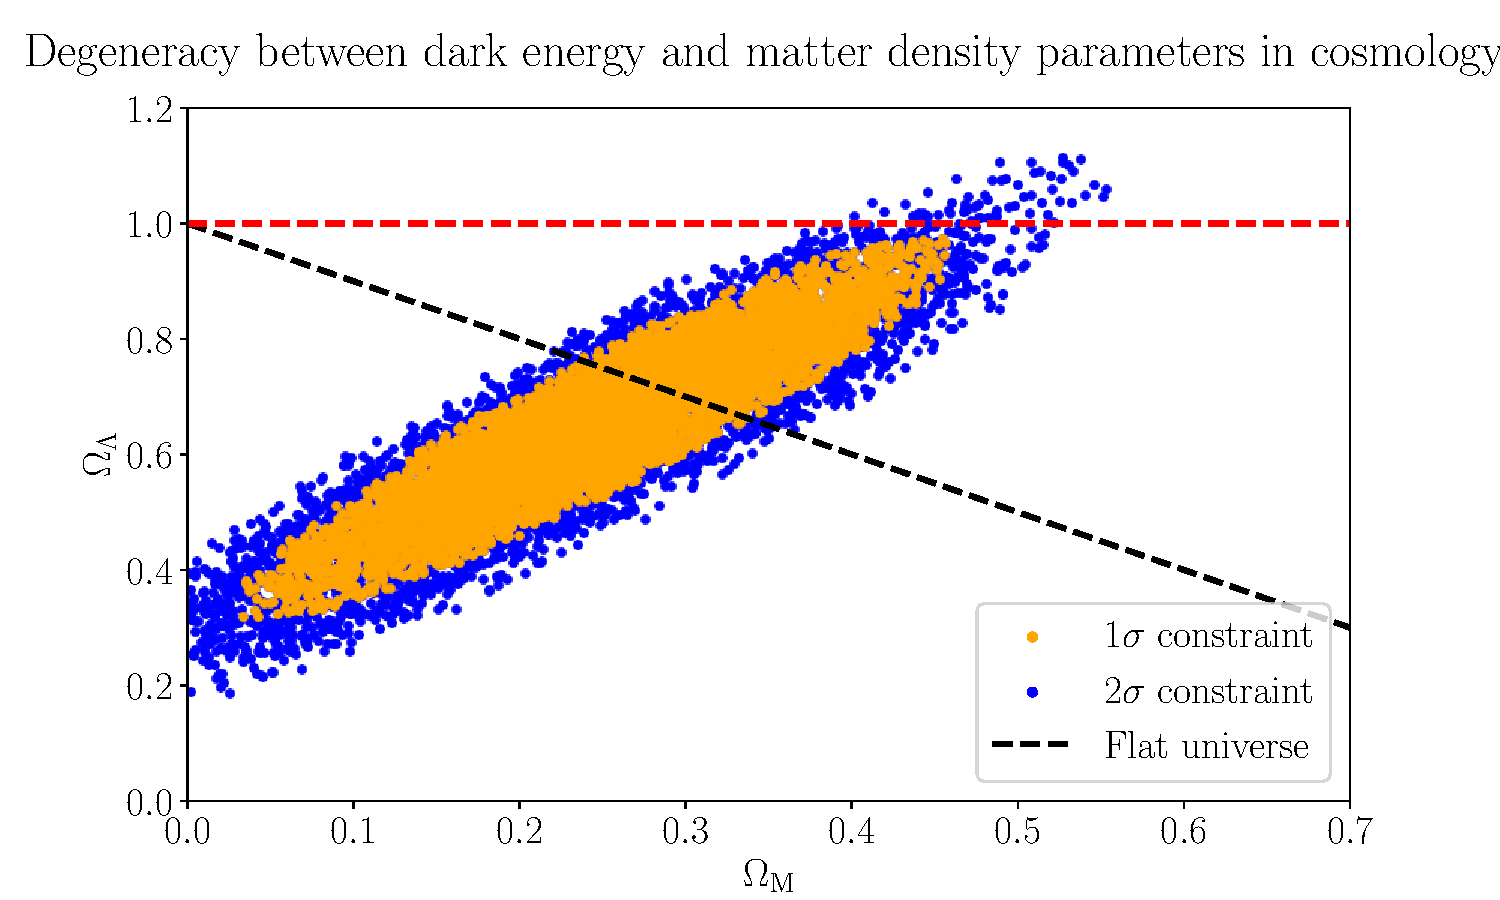
\includegraphics[width = \linewidth]{Figures/ScattPlot.pdf}
\caption{Supernova data with $1\sigma$ and $2\sigma$ constraints from MCMC fits.}
\label{fig:scatt}
\end{figure}





\subsection{Summary \& Conclusion}

To summarize this section, we numerically solved the ODEs for $\eta$ and $t$ past the radiation domination. We then computed $H(x)$ which gave us access to all the other relevant cosmological parameters. Further we checked that the numerical data corresponds to analytical approximations in the different regimes. Next we introduced all the most relevant data in a graphed form in FIG \ref{fig:TimeEvHp}-\ref{fig:PDEh} such that important events and values were easily visualized. The most relevant values for the most important events in our background cosmology were summarized in TABLE \ref{tab:cosmo_events}. Finally, an MCMC fit with observational data from supernova events and the numerical data in the $\Omega_{\Lambda}\Omega_{\text M}$-plane was made to consider some important aspects of our model, in particular that we cannot consider a model without dark energy. 

In conclusion, the data all seems to correspond quite well with observational data and previous calculations from more sophisticated methods.

\end{document}
